%%%%%%%%%%%%%%%%%%% EJERCICIO 10 %%%%%%
\textbf{Ejemplo 10}\\
¿Cuál es la tasa nominal anual (150 días) vencido equivalente a una tasa del 24\% 
periódica (200 días) anticipada? Asumir el año de 365 días.\\
%\newpage %USAR SOLO SI EL SOLUCIÓN QUEDA SOLO Y ES NECESARIO BAJARLO A LA SIGUIENTE PAGINA
\hfill
\textbf{Solución }\\
%La tabla ira centrada
\begin{center}
  \renewcommand{\arraystretch}{1.5}% Margenes de las celdas
  %Creación de la cuadricula de 2 columnas
  \begin{longtable}[H]{|c|c|c|}
    %Creamos una linea horizontal
    \hline
    %Definimos el color de la primera fila
    \rowcolor[HTML]{FFB183}
    %%%%% INICIO ASIGNACIÓN PERíODO FOCAL %%%%%%%
    %%%%%%%%%% INICIO TITULO

    %Lo que se hace aquí es mezclar las 3 columnas en una sola
      \multicolumn{3}{|c|}{\cellcolor[HTML]{FFB183}\textbf{1. Asignación período focal}}                                                                                                        \\ \hline
      \multicolumn{3}{|c|}{$pf= \textit{No aplica}$}                                                                                                                                              
      \\ \hline

    %%%%%%%%%% FIN TITULO
    %%%%% INICIO DECLARACIÓN DE VARIABLES %%%%%%%
    %%%%%%%%%% INICIO TITULO
    %Lo que se hace aquí es mezclar las 3 columnas en una sola
    \multicolumn{3}{|c|}{\cellcolor[HTML]{FFB183}\textbf{2. Declaración de variables}}                                                                 \\ \hline
    %%%%%%%%%% FIN TITULO
    %%%%%%%%%% INICIO DE MATEMÁTICAS
    %Cada & hace referencia al paso de la siguiente columna
    $j_{a1} = 24\% \textit{ na(200)da}$  &  $m_{1} =\frac{365días}{200días}= 1,82 \textit{ p(200)da}$  &  $i_{2} = ?\% \textit{ p(150)dv} $ \\ 
    
    $i_{a1}= 0,1319 \textit{ p(200)da} $ & $m_{2} = \frac{365días}{150días} = 2,43 \textit{ p(150)dv}$ & $j_{2} = ?\% \textit{ na(150)dv} $    \\                                                                                                     \hline
    %%%%%%%%%% FIN DE MATEMÁTICAS
    %%%%% FIN DECLARACIÓN DE VARIABLES

    %%%%% INICIO FLUJO DE CAJA
    \rowcolor[HTML]{FFB183}
    \multicolumn{3}{|c|}{\cellcolor[HTML]{FFB183}\textbf{3. Diagrama de equivalencia de tasas}}                                                        \\ \hline
    %Mezclamos 3 columnas y pondremos el dibujo
    %%%%%%%%%%%%% INSERCIÓN DE LA IMAGEN
    %Deberán descargar las imágenes respectivas del drive y pegarlas en la carpeta
    %n_capitulo/img/ejemplos/1/capitulo1ejemplo1.pdf  (el /1/ es el numero del ejemplo)

    \multicolumn{3}{|c|}{ 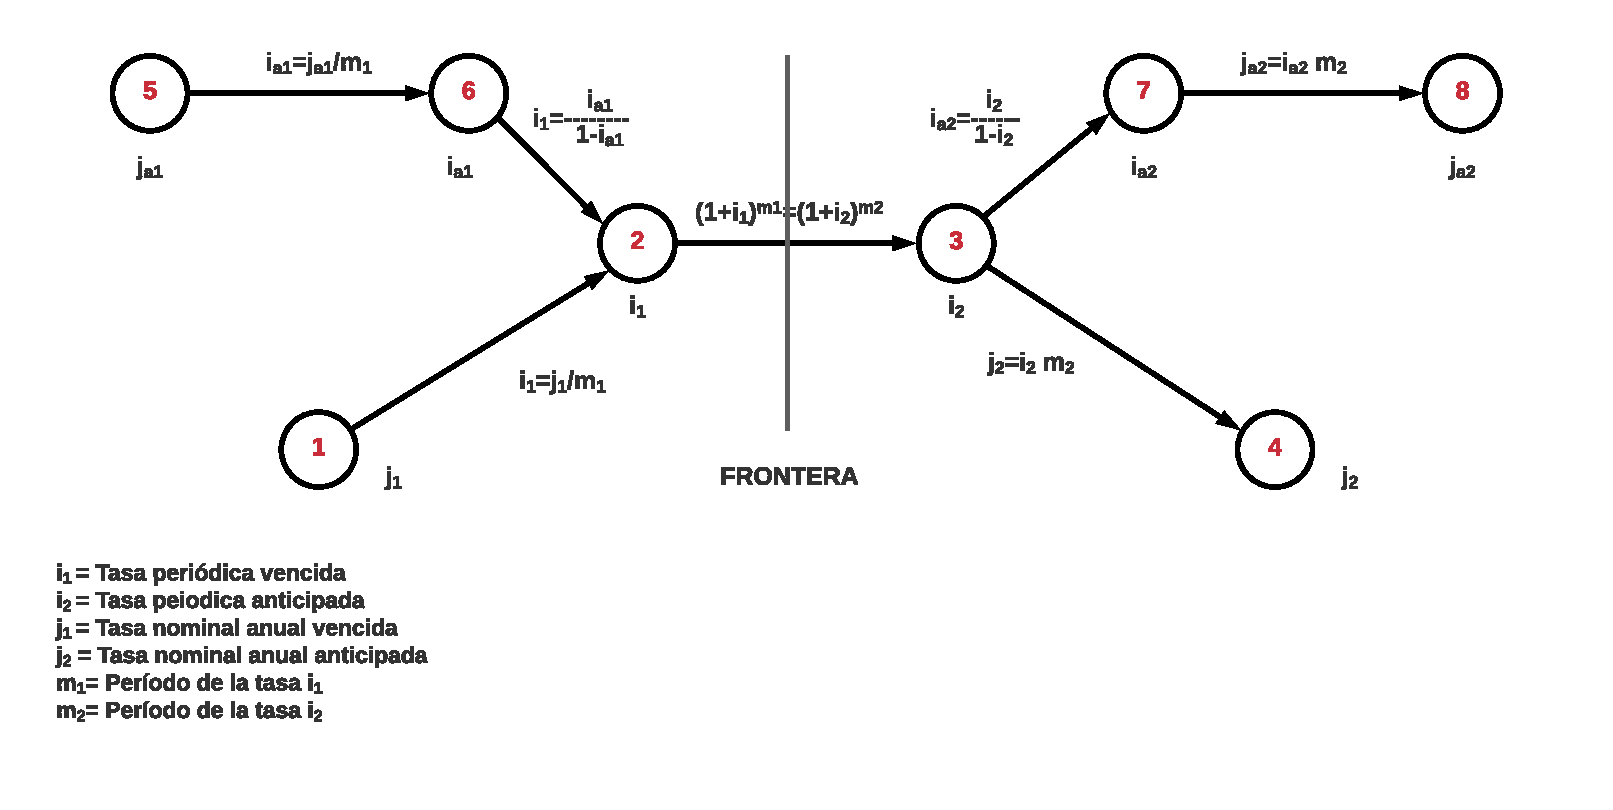
\includegraphics[trim=-5 -5 -5 -5 , scale=0.4]{2_Capitulo/img/ejemplos/6/Capitulo2Ejemplo6.pdf} } \\ \hline
    
    %%%%%%%%%%%%% FIN INSERCIÓN DE IMAGEN
    %%%%%FIN FLUJO DE CAJA

    %%%%% INICIO DECLARACIÓN FORMULAS
    %%%%%%%%%%% INICIO TITULO
    \rowcolor[HTML]{FFB183}
    \multicolumn{3}{|c|}{\cellcolor[HTML]{FFB183}\textbf{4. Declaración de fórmulas}}                                                                  \\ \hline
    %%%%%%%%%%% FIN TITULO
    %%%%%%%%%%% INICIO MATEMÁTICAS

    \multicolumn{2}{|c|} {$i_{1} = \frac{i_{1}}{1-{i_{a1}}} \textit{ Tasa periódica vencida }$} & {{\raggedleft  $j_{2}=i_{2}\cdot m_{2} \textit{ Tasa nominal anual vencida }$}} \\
    \multicolumn{2}{|c|} {$(1+i_{1})^{m_{1}}=(1+i_{2})^{m_{2}} \textit{ Equivalencia de tasas}$ }  & {$i_{a1} = \frac{j_{a1}}{m_{1}} \textit{ Tasa periódica anticipada}$}     \\ \hline
    %%%%%%%%%% FIN MATEMÁTICAS
    %%%%%% INICIO DESARROLLO MATEMÁTICO
    \rowcolor[HTML]{FFB183}
    %%%%%%%%%%INICIO TITULO
    \multicolumn{3}{|c|}{\cellcolor[HTML]{FFB183}\textbf{5. Desarrollo matemático}}                                                                    \\ \hline
    %%%%%%%%%% FIN TITULO
    %%%%%%%%%% INICIO MATEMÁTICAS
    \multicolumn{2}{|c|} {$i_{1} = \frac{0.1319}{1-0,1319} = 0,152 \textit{p(200)dv}$}   &  {$j_{2}=(11,18\% \textit{ p(150)dv})(2,43\textit{ p(150)dv})$}                            \\
    \multicolumn{2}{|c|} {$(1 + 0,152)^{1,82}= (1 + i_{2})^{2,43} $}  &  {\textit{$j_{2} = 27,17\% \textit{ na(150)dv}$}}                                                                          \\
    \multicolumn{2}{|c|} {$(1,152)^{\frac{1,82}{2,43}}-1=i_{2}$}  &                                                                            \\
    \multicolumn{2}{|c|} {$i_{2}=0,1118 \textit{ p(150)dv} \equiv 11,18\% \textit{ p(150)dv}$}                                   &                                                                                                   \\ 
    \hline
    %%%%%%%%%% FIN MATEMÁTICAS
    %%%%%% FIN DESARROLLO MATEMÁTICO
    %%%%%% INICIO RESPUESTA
    \rowcolor[HTML]{FFB183}
    %%%%%%%%%%INICIO TITULO
    \multicolumn{3}{|c|}{\cellcolor[HTML]{FFB183}\textbf{6. Respuesta}}                                                                                \\ \hline
    %%%%%%%%%% FIN TITULO
    %%%%%%%%%% INICIO RESPUESTA MATEMÁTICA
    \multicolumn{3}{|c|}{
         \begin{minipage}[t][0.03\textheight][c]{0.8\columnwidth}
            \centering
             ${j_{2} = 27,17\% na(150)dv}$
         \end{minipage}
      }  
    \\ \hline
    %%%%%%%%%% FIN MATEMÁTICAS
    %%%%%% FIN RESPUESTA
  \end{longtable}
  %Se crean dos lineas en blanco para que no quede el siguiente texto tan pegado
  %\newline \newline %USARLO SI CREES QUE ES NECESARIO
\end{center}
%%%%%%%%%%%%%%%%%%% FIN EJERCICIO 10  %%%%%%%%%%%%%%%%%%%%%%%%%%%%%%
